\subsection{Geheugenbeheer in UNIX en Solaris }

\textbf{Unix}

Was oorspronkelijk bedoelt om machine-onafhankelijk te zijn dus de implementaties verschillen:

\begin{itemize}
\item Eerdere UNIX: gebruikten gewoon een variabele partitionering zonder enige vorm van virtueel geheugen.
\item Recente UNIX (SVR4 en Solaris): gebruiken gepagineerd virtueel geheugen.
\end{itemize}

SVR4 gebruikt twee afzonderlijke systemen voor geheugenbeheer: 

Het pagineringssysteem en een kernelgeheugentoewijzing.

\subsubsection{Pagineringssysteem}

Het pagineringssysteem voorziet een virtueel geheugen mogelijkheid dat pagina frames in het hoofdgeheugen toekent aan processen. Het kent ook pagina frames toe aan harde schijf Block buffers.

\subsubsection{Kernelgeheugentoewijzing}

De kernelgeheugentoewijzing kent geheugen toe aan de kernel. Het pagineringssysteem is niet zo goed voor deze taak omdat de meeste van deze blokken aanzienlijk kleiner zijn dan de standaard paginagrootte.

\begin{figure}[htp]
    \centering
            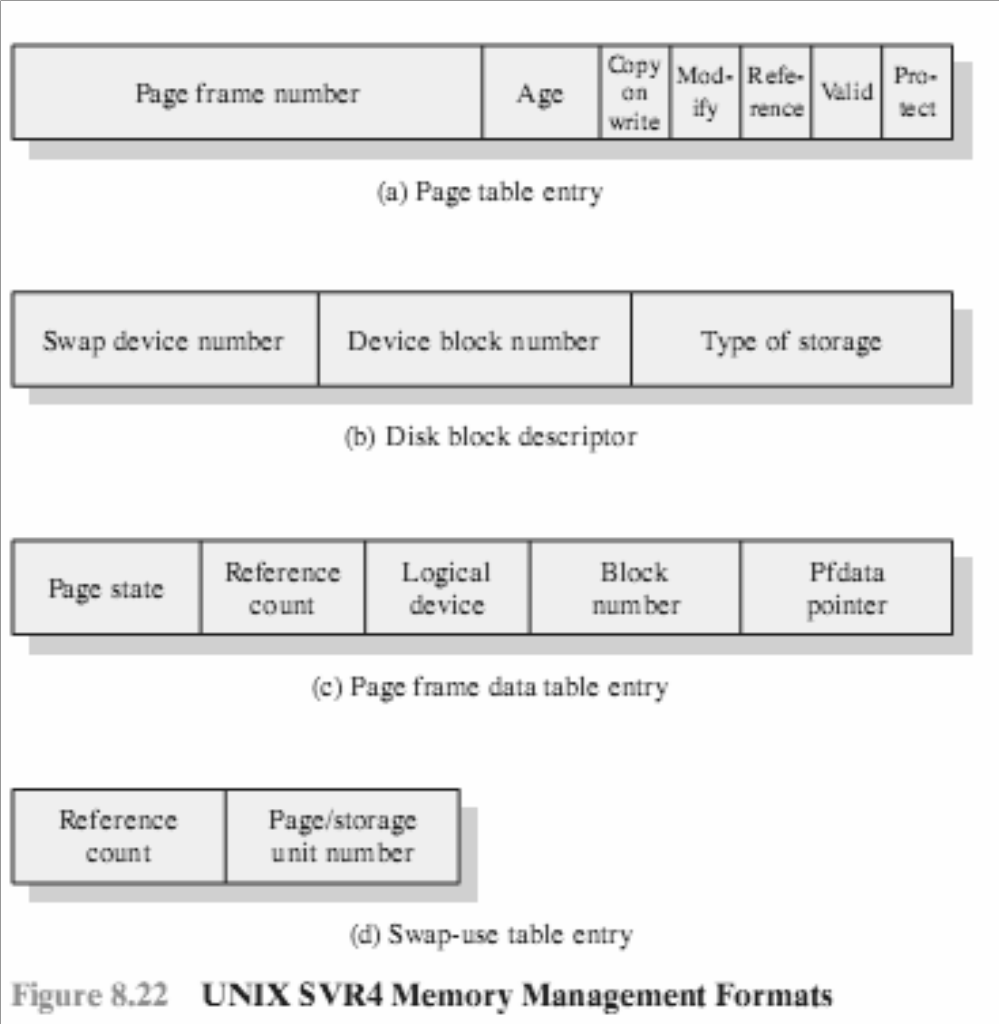
\includegraphics[width=4in]{img/Kernelgeheugentoewijzing}
        \caption{}
    \label{fig:}
\end{figure}

De paginaframegegevenstabel wordt gebruikt voor paginavervanging. Er worden verschillende wijzers gebruikt voor het maken van lijsten binnen deze tabel. Alle beschikbare frames zijn onderling gekoppeld in een lijst van vrije frames die beschikbaar zijn voor het binnenhalen van pagina’s. Daalt het aantal beschikbare pagina’s tot onder een bepaalde drempel, dan steelt de kernel ter compensatie enkele pagina’s.

Het algoritme gebruikt de referentie-bit in de paginatabelingang voor elke pagina in het geheugen die naar secundair geheugen mag worden geswapt. Deze bit is 0 wanneer de pagina voor het eerst wordt binnengehaald en wordt ingesteld op 1 wanneer de pagina wordt gerefereerd voor lezen of schrijven. Een wijzer (de voorste wijzer of fronthand), bladert door de pagina’s in de lijst met geschikte pagina’s en stelt de referentie-bit van elke pagina in op 0. Iets later bladert de achterste wijzer (backhand) door dezelfde lijst en controleert de referentie-bit. Is de bit 1, dan is naar de pagina verwezen sinds de fronthand is gepasseerd, is de bit 0 dan is er nog niet verwezen geweest naar de pagina sinds de fronthand is gepasseerd. De pagina’s met een 0, worden in een lijst geplaatst dat bestemd is voor swap-out.

\begin{figure}[htp]
    \centering
            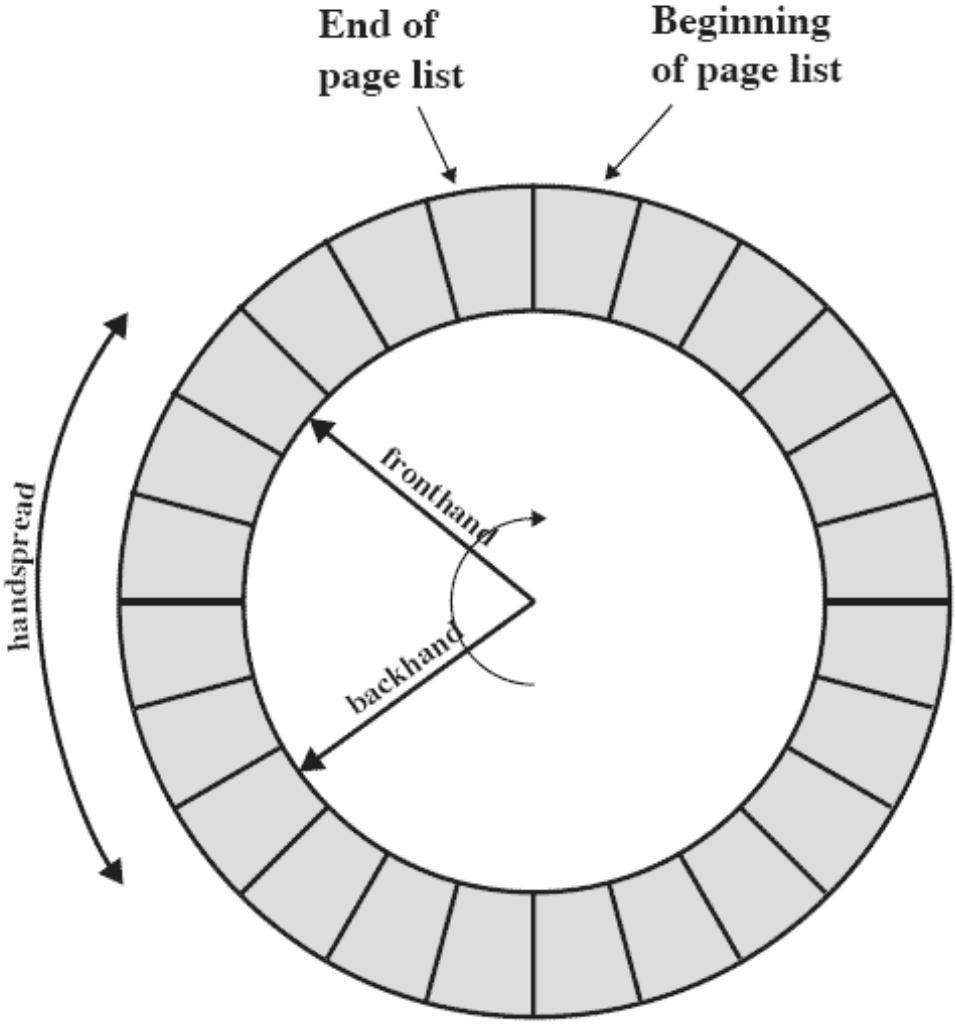
\includegraphics[width=4in]{img/klokalgoritme}
        \caption{Het klokalgoritme met twee wijzers.}
    \label{fig:Het klokalgoritme met twee wijzers.}
\end{figure}


\begin{itemize}
\item De zoeksnelheid (scanrate): de snelheid waarmee de twee wijzers de paginalijst doorzoeken, in pagina’s per seconde.
\item De wijzerspreiding (handspread): de ruimte tussen fronthand en backhand.
\end{itemize}


\subsubsection{Toewijzing van kernelgeheugen}

De kernel maakt en vernietigt kleine tables en buffers continu tijdens het uitvoeren van processen. Elke daarvan vereisen dynamische geheugentoewijzing.

Meeste blokken zijn veel smaller dan de typische pagina’s. Daarmee zou een normale pagineringssysteem inefficiënt zijn. Een variatie van het buddy-systeem wordt gebruikt.

De vraag om kernelgeheugen in UNIX vertoont vaak het gedrag van een stabiele toestand, met andere woorden: De vraag om blokken van een bepaalde grootte varieert langzaam in de tijd.

Om onnodige groepering en splitsing van blokken te vermijden, stelt het lazy buddy systeem het samenvoegen uit totdat het waarschijnlijk wordt dat samenvoegen noodzakelijk is, waarna het systeem zoveel mogelijk blokken samenvoegt.

Het Lazy Buddy systeem gebruikt de volgende parameters:

\begin{itemize}
\item $N_i$ = Aantal blokken van de grootte $2^i$
\item $A_i$ = Aantal blokken van de grootte $2^i$ die toegewezen (bezet) zijn
\item $G_i$ = Aantal blokken van de grootte $2^i$ die globaal vrij zijn, deze blokken komen in aanmerking voor groepering.
\item $L_i$ = Aantal blokken van de grootte $2^i$ die lokaal vrij zijn, deze blokken komen niet in aanmerking voor groepering.
\end{itemize}
Merk op!! : $N_i = A_i + G_i  + L_i$

\begin{figure}[htp]
    \centering
            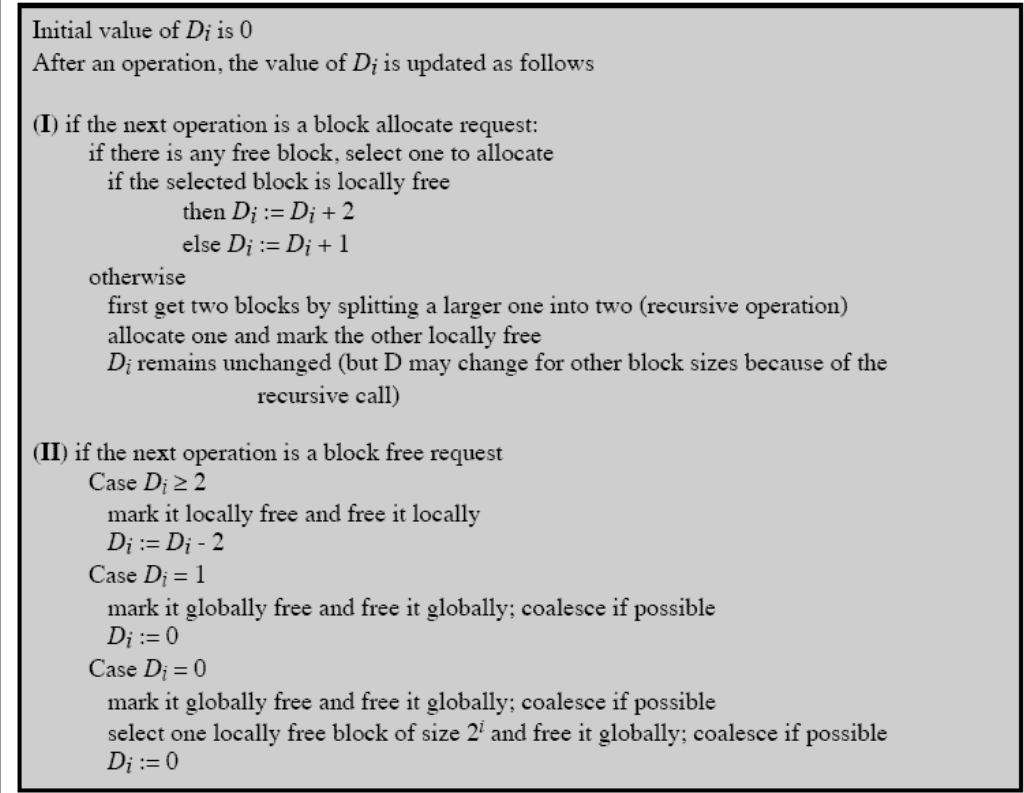
\includegraphics[width=4in]{img/lazybuddy}
        \caption{Lazy Buddy algoritme:}
    \label{fig:Lazy Buddy algoritme:}
\end{figure}